% \clearpage

\section{Detecção de Novidade}\label{sec:nd}

\newcommand{\novelty}{\emph{Novelty Detection}\xspace}
\newcommand{\drift}{\emph{Concept Drift}\xspace}
\newcommand{\evolution}{\emph{Concept Evolution}\xspace}

% \notafa{(senteça marcada) Alguns autores consideram novidade e anomalia como a
% mesma coisa. Outros não (eu sou um dos que não considera)}
No âmbito de classificação de dados, parte da área de aprendizado de máquina, os
métodos de detecção de novidade (\novelty, \nd) lidam com o reconhecimento e a 
classificação \hlke{de exemplos que diferem de
exemplos anteriores} \cite{PERNER2007,Gama2010}.
Esses métodos tratam da classificação em fluxos de dados que evoluem com o
tempo, levando em consideração as características desse tipo de fluxos.

% \nota{"As características desse tipo de fluxo de dados são?".. mas que tipo?}

Tratando-se de fluxos de dados contínuos, são características
\notahl{quais?}dos \hlhl{padrões observados}:
evolução de conceito (\evolution) em que novos padrões podem surgir;
desaparecimento ou recorrência de conceito, em que padrões podem desaparecer e
também podem reaparecer;
mudança de conceito (\drift, também nomeado deriva ou desvio) onde um padrão
gradualmente se transforma;
presença de ruído e \emph{outliers} \cite{Gama2010}.

% \nota{separar ai - ndpara\\
% padroes novidade? reconhecomemnto de padroes novidade?}

Os métodos de \nd são aplicados a diversos problemas como
detecção de intrusos \cite{Coull2003,Spinosa2008,Viegas2019,Cassales2019a},
detecção de falhas \cite{Zhang2006},
diagnósticos médicos \cite{Perner2009},
detecção de regiões de interesse em imagens \cite{singh2004approach},
detecção de fraudes \cite{wang2003mining,Abdallah201690}, 
filtros de spam \cite{Hayat2010dct} e
detecção de variações comportamentais em um jogador \cite{Vallim20136258}.

% breve descrição do que sao algoritmos para DN

\nota{TODO: terminar reescrita}
Alguns métodos de \nd utilizam 
\notafa{frase estranha}
tratam de novidades como uma classificação de uma
ou duas classes () onde um conceito representa a classe normal e
as 
\hlfa{anomalias são representadas}
\hlfa{pela falta de conceito no modelo} ou
como um segundo conceito no modelo.
Além da abordagem de classificação binária, 
% não é adequada para representar
% \notafa{alguns trabalhos fazem isso, mas nem todos. É importante destacar que
% isso é a visão de um grupo de autor.}
\hlfa{múltiplos conceitos}
em um mesmo conjunto de dados, para isso é necessário abordar
\nd como classificação multi-classe.
Alguns métodos que abordam \nd como classificação multi-classe não
atendem completamente características de conjuntos com 
\notafa{o que é evolução temporal?}
\hlfa{evolução temporal,}
como \evolution e \drift, deixando de detectar múltiplos padrões que surgem
simultaneamente num intervalo de avaliação \cite{Faria2016nd,Gama2010}.

% \notafa{um grupo de algoritmos fazem isso, mas nem todos}
A maioria dos métodos de \nd são construídos seguindo a abordagem de aprendizado
\emph{Offline-Online}. Essa abordagem estabelece que o método seja dividido em
duas fases:
a primeira fase (\emph{Offline}) usa um conjunto de exemplos rotulados para
deles extrair conceitos conhecidos e gerar um modelo;
a segunda fase (\emph{Online}) consome um conjunto ou fluxo de exemplos não
rotulados e detecta padrões-novidade.
Além de detectar padrões-novidade, alguns algoritmos classificam cada exemplo
em um dos conceitos do modelo, ou marca o exemplo como desconhecido.
Ainda na segunda fase, para atualizar o modelo, os exemplos marcados como
desconhecidos são utilizados para a extração de novos conceitos ou variações em
conceitos conhecidos \cite{Gama2010}.

Dentre os métodos de \nd que baseiam-se em aprendizado \emph{Offline-Online},
muitos são baseados em algoritmos de agrupamento não supervisionados, tanto
para construção do modelo inicial como na extração de novos conceitos dos
exemplos não explicados pelo modelo marcados como desconhecidos
\cite{Spinosa2009ollinda,Masud2010ECSMiner,Faria2013}.

% Essa abordagem se deve as características 

% \cite{Gama2007,Gama2010,Masud2010ECSMiner,Faria2013,Lavin2015,Abdallah2016anynovel}.

% \cite{Costa2019thesis}

%     - técnicas de Detecção de novidades
% ver se tem algum survey e citar
% (PERNER, 2007)(GAMA, 2010)
% ECSMiner (MASUD et al., 2011)

\subsection{O algoritmo MINAS}\label{sec:minas-og}

Um algoritmo de \nd que tem recebido atenção nos últimos anos é o algoritmo
MINAS, originalmente proposto por \citeonline{Faria2013}, refinado por
\citeonline{Faria2015minas} e recentemente aprimorado por
\citeonline{DaSilva2018thesis}, com o uso de conceitos \emph{Fuzzy}, e expandido por
\citeonline{Costa2019thesis}, para tratar problemas multi-rótulo além dos problemas
multi-classe já tratados na versão original.
Esse algoritmo segue a abordagem de duas fases no modelo \emph{Offline-Online} e
usa por base algoritmos de agrupamento não supervisionados como \emph{K-means} e
\emph{CluStream}.
% As duas fases, com exceção do método de detecção de padrões novidade da fase
% \emph{Online}, são ilustradas na \reffig{minas}.

% \begin{figure}[ht]
% \centering
% 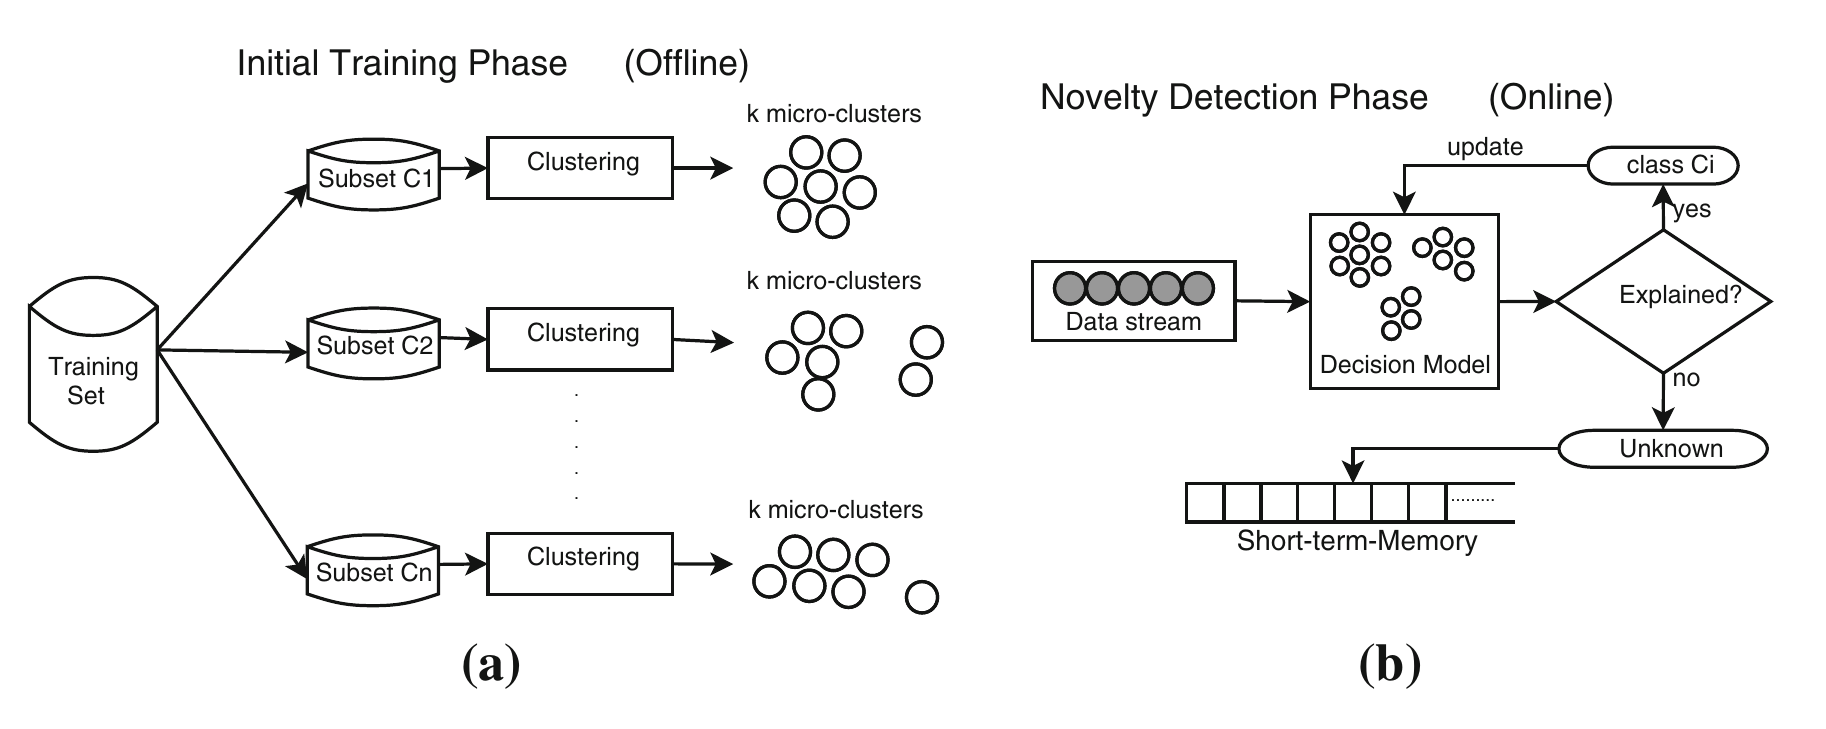
\includegraphics[width=1\textwidth]{figuras/FariaMinas2015-fases.png}
% \caption{Visão geral do algoritmo MINAS com fases \emph{Offline} (a) e 
% \emph{Online} (b) \cite{Faria2015minas}}
% \label{fig:minas}
% \end{figure}

\newcommand{\mcluster}{\emph{micro-cluster}\xspace}
\newcommand{\mclusters}{\emph{micro-clusters}\xspace}

% \nota{talvez mencionar que o minas trabalha no dominio de Double[]}

O algoritmo MINAS em sua fase \emph{Offline} consome um conjunto de treinamento
contendo exemplos etiquetados.
Esse conjunto de treinamento é dividido em grupos usando como chave a etiqueta,
e para cada grupo de exemplos o método de agrupamento (\emph{clustering}) é executado.
O método de agrupamento objetiva resumir um conjunto maior de exemplos em
um conjunto menor de \mclusters.

% \notafa{essas estatisitcas podem ser deduzidas pelos sumario, mas nao sao o sumario}
Um \mcluster é uma tupla de quatro components $(N, \mathbf{LS}, \mathbf{SS}, T)$
derivados dos exemplos representados por este \mcluster, onde:
$N$ número de exemplos,
$\mathbf{LS}$ soma linear dos exemplos,
$\mathbf{SS}$ soma quadrada dos exemplos,
$T$ instante de chegada do último exemplo adicionado ao \mcluster.
Deste sumário extrai-se, entre outras estatísticas, o centro e raio que são
utilizados na operação de classificação da fase \emph{Online}.
A cada \mcluster é adicionada a etiqueta do grupo original e todos \mclusters
são arranjados em um único conjunto formando o modelo de decisão.

Na fase \emph{Online}, listada no Algoritmo \ref{alg:MINAS}, o algoritmo MINAS
opera com três operações: classificação de novos exemplos, detecção de 
padrões-novidade e atualização do modelo de decisão \cite{Faria2015minas}.
O primeiro método é o de classificação, onde exemplos do fluxo de dados
são consumidos e avaliados pelo modelo de decisão.
O modelo de decisão avalia cada exemplo calculando a distância euclidiana
entre o exemplo e todos \mclusters do modelo, selecionando o
\mcluster de menor distância.
Se a distância entre o exemplo e o centro do \mcluster for menor que
o raio do \mcluster, o exemplo é classificado com a etiqueta do \mcluster
e o sumário estatístico do \mcluster é atualizado.
Caso a distância (mínima no modelo) seja maior que o raio,
o exemplo é marcado como desconhecido e armazenado
em conjunto próprio \cite{Faria2015minas}.

O segundo método da fase \emph{Online} é a detecção de padrões novidade,
que é executada quando o tamanho do conjunto de desconhecidos é maior
que um parâmetro predefinido.
Esse método executa o agrupamento (\emph{clustering} descrito na fase
\emph{Offline}) e valida os \mclusters gerados verificando sua representatividade
e coesão.

\subsection{MINAS}
\label{sec:minas}

\minas \cite{Faria2013Minas,Faria2015minas} is an offline-online \nd algorithm,
meaning it has two distinct phases. The first phase (offline) creates an initial
model set with several clusters based on a clustering algorithm with a training
set.
Each cluster can be associated with only one class of the problem, but each
class can have many clusters.

During its online phase, which is the main focus of our work, \minas performs
three tasks in (near) real-time,
in summary,
classification, novelty detection, and model update tasks
in a potentially infinite data stream, as shown in Algorithm \ref{alg:minas-main}.

\minas attempts to classify each incoming unlabeled instance according to the
current decision model. Instances not explained by the current model
receive an \textit{unknown} label and are stored in an unknowns-buffer.
When the unknowns-buffer reaches a preset threshold, \minas executes the
Novelty Detection function.
After a set interval, samples in the unknowns-buffer are considered to be
noise or outliers and removed.
The algorithm also has a mechanism to forget clusters that became obsolete and
unrepresentative of the current data stream distribution, removing them from
the Model and storing in a Sleep Model for possible recurring pattern
detection \cite{Faria2015minas}.

\begin{algorithm}[htb]
    % \DontPrintSemicolon
    \SetKwFunction{nearestCluster}{nearestCluster}
    \SetKwFunction{clustering}{clustering}
    \SetKwFunction{NoveltyDetection}{NoveltyDetection}
    \SetKwFunction{handleModelSleep}{moveToSleep}
    \SetKwFunction{removeOldSamples}{removeOldSamples}
    % 
    \SetKwProg{Function}{Function}{:}{}
    \SetKwFor{With}{with}{}{}
    \SetKw{continue}{continue}
    % 
    \KwIn{ModelSet, inputStream}
    \KwOut{outputStream}
    % 
    \SetKwData{cleaningWindow}{cleaningWindow}
    \SetKwData{noveltyDetectionTrigger}{noveltyDetectionTrigger}
    \SetKwInOut{KwParams}{Parameters}
    \KwParams{\cleaningWindow, \noveltyDetectionTrigger}
    % \KwSty{Parameters}: \cleaningWindow, \noveltyDetectionTrigger\\
    % 
    \SetKwFunction{MinasOnline}{MinasOnline}
    \Function{\MinasOnline{ModelSet, inputStream}}{
        UnkownSet $\leftarrow$ $\emptyset$, ModelSleepSet $\leftarrow$ $\emptyset$ \;
        lastCleanup $\leftarrow 0$ , noveltyIndex $\leftarrow 0$\;
        % sampleIn $\leftarrow 0$\;
        \ForEach{ {$sample_{i}$} $\in$ inputStream }{
            % sample.label $\leftarrow$ unknown\;
            % (distance, cluster) $\leftarrow$ \nearestCluster(sample, ModelSet)\;
            nearest $\leftarrow$ \nearestCluster(sample, ModelSet)\;
            \eIf{nearest.distance $<$ nearest.cluster.radius}{
                sample.label $\leftarrow$ nearest.cluster.label\;
                nearest.cluster.lastUsed $ \leftarrow i $ \;
            }
            {
                sample.label $\leftarrow$ unknown\;
                UnkownSet $\leftarrow$ UnkownSet $\cup$ sample\;
                \If{$|\;UnkownSet\;| \geq$ \noveltyDetectionTrigger}{
                    % \tcc{Novelty Detection}
                    novelties $\leftarrow$ \NoveltyDetection(ModelSet $\cup$ ModelSleepSet, *UnkownSet)\;
                    ModelSet $\leftarrow$ ModelSet $\cup$ novelties\;
                }
                \If{ $ i > $ ( lastCleanup $ + $ \cleaningWindow )}{
                    ModelSet $\leftarrow$ \handleModelSleep(ModelSet, *ModelSleepSet, lastCleanup)\;
                    UnkownSet $\leftarrow$ \removeOldSamples(UnkownSet, lastCleanup)\;
                    lastCleanup $ \leftarrow i $\;
                }
            }
            outputStream.append(sample)\;
        }
    }
\caption{Our interpretation of \minas baseado em \cite{Faria2015minas}}
\label{alg:minas-main}
\end{algorithm}

The Novelty Detection function, illustrated in Algorithm \ref{alg:MINAS-nd},
groups the instances to form new clusters, and each new cluster is validated to
discard the non-cohesive or unrepresentative ones.
Valid clusters are analyzed to decide if they represent an extension of a
known pattern or a completely new pattern. In both cases, the model absorbs the
valid clusters and starts using them to classify new instances.

\begin{algorithm}[htb]
    \SetKwProg{Function}{Function}{:}{}
    \SetKwData{minExamplesPerCluster}{minExamplesPerCluster}
    \SetKwData{noveltyFactor}{noveltyFactor}
    \SetKwInOut{KwParams}{Parameters}
    \KwParams{\minExamplesPerCluster, \noveltyFactor}
    % 
    \SetKwFunction{nearestCluster}{nearestCluster}
    \SetKwFunction{clustering}{clustering}
    \SetKwFunction{NoveltyDetection}{NoveltyDetection}
    \SetKwFunction{handleModelSleep}{moveToSleep}
    \SetKwFunction{removeOldSamples}{removeOldSamples}
    % 
    \Function{\NoveltyDetection{Model, Unknowns}}{
        newModelSet $\leftarrow$ $\emptyset$\;
        \ForEach{cl in \clustering(Unknowns)}{
            \If{$|\;cl.sampleSet\;| \geq$ \minExamplesPerCluster}{
                (distance, near) $\leftarrow$ \nearestCluster(cl, Model)\;
                \eIf{distance $<$ near.radius $\times$ \noveltyFactor}{
                    cl.label $\leftarrow$ near.label\;
                    cl.type $\leftarrow$ extension\;
                }{
                    cl.label $\leftarrow$ noveltyIndex\;
                    noveltyIndex $\leftarrow$ noveltyIndex $+ 1$\;
                    cl.type $\leftarrow$ novelty\;
                }
                Unknowns $\leftarrow$ Unknowns $-$ cl.sampleSet\;
                \label{alg:MINAS-nd:reclassify}
                newModelSet $\leftarrow$ newModelSet $\cup$ cl\;
            }
        }
        \Return{newModelSet}\;
    }
    \caption{\minas \cite{Faria2015minas} Novelty Detection task.}
    \label{alg:MINAS-nd}
\end{algorithm}

Para atribuição de etiquetas aos \mclusters gerados, o algoritmo MINAS
encontra no modelo atual o \mcluster mais próximo pela distância
euclidiana e classifica em dois tipos de conceito.
Se a distância é menor que um parâmetro predefinido,
o novo \mcluster gerado recebe como etiqueta o valor de extensão
de conceito conhecido.
Caso contrário, se o novo \mcluster está mais distante,
um novo conceito foi encontrado e a etiqueta marca um padrão novidade.
Após a atribuição da etiqueta do novo \mcluster, ele é adicionado
ao modelo de decisão.

% Although efficient in detecting NP, MINAS is
% very sensitive to noisy data and data scale, what causes a
% decrease in its accuracy. \cite{DaSilva2018}

% ver paper da profa. Elaine

% % discussão de 2020-02-01
% Detecção de intrusão em redes
%     - riscos de segurança
%     % pontos de coleta de dados básicos para a maioria das estruturas de IoT sao Wireless Sensor Networks (WSN) e WSN baseadas em IP,
%     % as quais s˜ao vulneráveis e geram uma ameac¸a de seguranc¸a de alto n´ıvel (ADAT; GUPTA, 2018) Adat2018
%     % (KASINATHAN et al., 2013), a detecc¸ ˜ao de assinaturas
%     % (RAZA; WALLGREN; VOIGT, 2013; SHEIKHAN; BOSTANI, 2016) s˜ao propostos IDSs h´ıbridos com foco 
%                 % espec´ıfico em ataques de roteamento como sink-hole e redireciona- mento seletivo
%     - técnicas de intrusão e tipos de ataques
%     - mecanismo de detecção (análise de fluxo de rede -> detecção de anomalia)
%     % Guilherme: A tarefa de detecção de intrusão consiste em descobrir, 
%     %           determinar e identificar a utilização, duplicação, alteração ou destruição
%     %           não autorizada de sistemas de informação (MUKKAMALA; SUNG; ABRAHAM, 2005) Mukkamala2005
%     % deteccao por assinaturas (tambem chamada de misuse-detection), deteccao comportamental (tambem chamada de anomaly-detection)e deteccao hıbrida.(MODI et al., 2013).
%     % implementacao usualmente é feita por meio de técnicas de AM e MD (BUCZAK; GUVEN, 2016).
%     % existem poucos trabalhos [..] online e deteccao de novidade ao problema [..] observado nas surveys (BUCZAK; GUVEN, 2016; MITCHELL; CHEN, 2014; MODI et al., 2013).
%     % (FURQUIM et al., 2018), os autores implementam uma arquitetura de 3 camadas (WSN, Fog e Cloud)
%     % (MIDI et al., 2017), os autores propuseram um IDS h´ıbrido [...] ativa apenas os módulos [...] especializado em um ataque espec´ıfic
%     % (FAISAL et al., 2015)externo ou interno ao Smart Meter.dados do KDD99 [...] precis˜ao, Kappa, consumo de memória, tempo e FAR
%     % extensivamente em (Sommer; Paxson, 2010) e (MCHUGH, 2000), é dif´ıcil encontrar boas me- didas de avaliac¸ ˜ao para IDSs
%     % (GAMA, 2010) afirma que no contexto de processamento de fluxo, as medidas tradicionais s˜ao impreci- sas.
% Detecção de novidades
%     % (PERNER, 2007)(GAMA, 2010). A
%     - técnicas de Detecção de novidades
%     - MINAS (incluir métricas) 
%     % (FARIA et al., 2016)
%     % ECSMiner (MASUD et al., 2011)
%     % AnyNovel (ABDALLAH et al., 2016) s˜ao
%     % medidas de Qualidade da Deteccao utilizadas foram Fnew, Mnew, Erro e a quantidade de exemplos rotulados por especialistas que cada técnica requisitou (MASUD et al., 2011)
%     - BigFlow (incluir métricas)
% Processamento de Streams (big data)
%     - cloud?
%     % A arquitetura Lambda (MARZ; WARREN, 2015) de duas camadas de CPU (stream e batch) e camada de serviço
%     % Kappa (KREPS, 2014) possui apenas um módulo de processamento on-line (apenas as camadas de processamento e servic¸o)
%     - redes como stream
%     - Atraso
%     - Kafka/Spark/Flink
% Redes IoT
%     - Restrição hardware (Energia, CPU, Mem, Rede)
%     - Consideração FOG vs Cloud
% %/discussão


% \subsection{Algoritmos de Detecção de Novidades}\label{sec:alg-nd}

\newcommand{\cluster}{\emph{cluster}\xspace}
\newcommand{\clusters}{\emph{clusters}\xspace}

\newcommand{\dataset}{\emph{data set}\xspace}
\newcommand{\datasets}{\emph{data sets}\xspace}
% \clusters é um conjunto de \cluster feito de um \dataset.

O algoritmo MINAS, como já foi discutido na Seção \ref{sec:minas-og}, classifica
exemplos e detecta
novidades em DS e considera em sua composição \emph{concept drift} e
\emph{concept evolution}, sendo capaz de classificar como extensão de classe
conhecida e identificar padrões novidade sem intervenção de especialista
\cite{Faria2015minas}.
Neste trabalho, consideram-se algoritmos derivados do algoritmo MINAS
aqueles apresentados em trabalhos publicados após 2016, que estendem a
implementação original seguindo sua estrutura básica.

\subsection{Algoritmo FuzzyND}

% FuzzyND
% $(n, \mathit{M}, \overline{CF1^x}, SSD^e, t, l)$
% $(n, LS, SS, t, l)$
% A nova estrutura contrapõem a estrutura original
% substituindo a soma linear dos elementos ($LS$) por  e $SS$ por $M$ e $$

O algoritmo FuzzyND, derivado do MINAS foi proposto por \citeonline{DaSilva2018}.
FuzzyND incrementa o algoritmo original, aplicando a ele teorias de
conjuntos \emph{fuzzy} pela modificação da representação dos \clusters.
A modificação afeta o método de construção de \clusters, método de classificação
de exemplos e método de detecção de novidades de acordo com a nova representação.

\acronym{F1M}{\emph{Macro F-Score}, acurácia }

A avaliação do algoritmo FuzzyND foi feita por meio de experimentos usando 3 
\datasets sintéticos (\emph{MOA3}, \emph{RBF}, \emph{SynEDC})
e por comparação com o MINAS.
O método de avaliação utilizado baseia-se na matriz de confusão incremental
descrita por \citeonline{Faria2016nd}, extraindo dessa matriz duas métricas:
acurácia (\emph{Macro F-Score}) \cite{Sokolova2009} e
taxa de desconhecidos (\emph{UnkR}) \cite{Faria2015minas}.
Em geral, o algoritmo FuzzyND detecta melhor novidades e, consequentemente,
é mais robusto a valores atípicos (\emph{outlier}), porém perde a capacidade
de reconhecer padrões recorrentes.


% Experiments were evaluated using the incremental confusion-matrix proposed by [27],
% recently been proposed [5]–[9]
% [5] T. Al-Khateeb, M. M. Masud, L. Khan, C. Aggarwal, J. Han, and B.
% Thuraisingham, “Stream classification with recurring and novel class detection
% using class-based ensemble,” in Data Mining (ICDM), 2012 IEEE 12th International
% Conference on. IEEE, 2012, pp. 31–40.
% [6] E. R. de Faria, A. C. P. de Leon Ferreira, J. Gama et al., “Minas:
% multiclass learning algorithm for novelty detection in data streams,” Data
% Mining and Knowledge Discovery, vol. 30, no. 3, pp. 640–680, 2016.
% [7] M. Masud, J. Gao, L. Khan, J. Han, and B. M. Thuraisingham, “Classification
% and novel class detection in concept-drifting data streams under time
% constraints,” IEEE Transactions on Knowledge and Data Engineering, vol. 23, no.
% 6, pp. 859–874, 2011.
% [8] M. M. Masud, Q. Chen, L. Khan, C. Aggarwal, J. Gao, J. Han, and B.
% Thuraisingham, “Addressing concept-evolution in concept-drifting data streams,”
% in Data Mining (ICDM), 2010 IEEE 10th International Conference on. IEEE, 2010,
% pp. 929–934.
% [9] Z. S. Abdallah, M. M. Gaber, B. Srinivasan, and S. Krishnaswamy, “Anynovel:
% detection of novel concepts in evolving data streams,” Evolving Systems, vol. 7,
% no. 2, pp. 73–93, 2016.
% [27] E. R. de Faria, I. R. Goncalves, J. Gama, A. C. P. de Leon Ferreira et al.,
% “Evaluation of multiclass novelty detection algorithms for data streams,” IEEE
% Transactions on Knowledge and Data Engineering, vol. 27, no. 11, pp. 2961–2973,
% 2015.
% [28] M. Sokolova and G. Lapalme, “A systematic analysis of performance measures
% for classification tasks,” Information Processing & Manage- ment, vol. 45, no.
% 4, pp. 427–437, 2009.

\subsection{Algoritmos MINAS-LC e MINAS-BR}\label{sub:minas-derivados}

O algoritmo MINAS-LC foi proposto por \citeonline{Costa2019thesis} e trata a classificação
multi-rótulo, porém não trata evoluções de conceito (\emph{Concept Evolution}).
As alterações fundamentais propostas são:
a representação de \cluster onde MINAS-LC troca a etiqueta, que era única, por uma multi-rótulo;
a transformação de problema aplicada ao conjunto de treinamento para transformá-lo de um
conjunto multi-rótulo para um conjunto multi-classe (simplificação)
em duas variações \emph{Label Powerset} e \emph{Pruned Sets} com
mineração de conjunto de itens frequentes.

% Este capítulo apresentou o método MultI-label learNing Algorithm for data
% Streams with Label Combination-based methods (MINAS-LC) e o MultI-label learNing
% Algorithm for data Streams with Binary Relevance transformation (MINAS-BR) para
% CMFCD com latência extrema de rótulos. O MINAS-LC lida com problemas apenas com
% mudanças de conceito. O seu modelo de decisão e composto por microgrupos
% multirrotulados sendo capaz de classificar exemplos em várias classes
% simultaneamente e evoluir ao longo do fluxo de dados. Foram propostas duas
% variações do método: utilizando o método de transformação de problema Label
% Powerset (LP) e, utilizando o método Pruned Sets (PS) com mineração de conjunto
% de itens frequentes. O MINAS-BR lida com problemas tanto com mudanças de
% conceito, como com evo- luções de conceito. Ele possui um conjunto de modelos de
% decisão, um para cada classe do problema. Esses modelos de decisão podem ser
% entendidos adaptando-se às mudanças de con- ceito, ou novos modelos de decisão
% podem ser criados, adaptando-se às evoluções de conceito. O próximo capítulo
% apresenta os experimentos realizados envolvendo os dois métodos propostos neste
% trabalho.

Já o trabalho de \citeonline{Costa2019}, estende o algoritmo original para que
classifique um exemplo com uma ou mais etiquetas usando a transformação
\emph{Binary Relevance}, o que deu origem ao algoritmo MINAS-BR.
O algoritmo modifica a representação do modelo, originalmente conjunto de \clusters, para
um grupo de \clusters por classe (etiqueta).
Também modifica o método de agrupamento, substituindo a inicialização do 
algoritmo \emph{K-means}, originalmente aleatória, pelo algoritmo 
\emph{Leader Incremental Clustering} \cite{Vijaya2004505}.

% as 4CRE-V13, 4CRE-V24 e 5CVT5 6 foram geradas originalmente em Souza et al. (2015b)
% SOUZA, V. M. A.; SILVA, D. F.; GAMA, J.; BATISTA, G. E. A. P. A. Data stream
% classification guided by clustering on nonstationary environments and extreme
% verification latency. In: Procee- dings ofSIAM International Conference on Data
% Mining (SDM). [S.l.: s.n.], 2015. p. 873–881. Citado 4 vezes nas páginas 17, 65,
% 87 e 89.

O algoritmo MINAS-BR também é experimentalmente avaliado com 4 \emph{data sets}
sintéticos: \emph{MOA-3C-5C-2D}, \emph{MOA-5C-7C-2D}, \emph{MOA-5C-7C-3} da
ferramenta MOA \cite{MOA} e \emph{4CRE-V2}
\footnote{
    A versão original do \dataset 4CRE-V2 está disponível em
    \url{https://sites.google.com/site/nonstationaryarchive/home}
}
gerados pelo método \emph{Radial Basis Function} \cite{souza2015,Costa2019}.
O algoritmo MINAS-BR foi comparado com 7 algoritmos da literatura também
disponíveis na ferramenta MOA \cite{MOA}, diferente da avaliação do FuzzyND que
compara diretamente com MINAS. Para análise, os 7 algoritmos foram divididos em
dois grupos \cite{Costa2019}.
O primeiro grupo de 3 algoritmos com acesso às etiquetas corretas para
atualização do modelo e com a técnica ADWIN (\emph{ADaptive WINdowing}) para detectar
mudanças de conceito (\emph{Concept Drift})
O segundo grupo com os 4 algoritmos sem acesso às etiquetas corretas,
ou seja, sem \emph{feedback} externo, mesma condição do MINAS-BR \cite{Costa2019}.

% Esse trecho parece mais fundamentação.

A avaliação elencada por \citeonline{Costa2019} leva em consideração que as classes
contidas no conjunto de testes podem não ter correlação direta com os padrões identificados
pelos algoritmos.
Para tratar a divergência, uma estratégia baseada em proposta anterior por
\citeonline{Faria2016nd} foi apresentada com alterações para exemplos multi-rótulo.
Após associação entre padrões de novidade e classes novidade foi possível calcular
métricas tradicionais.
A estratégia é executada na fase de classificação seguindo as regras:

\begin{enumerate}

    \item após o consumo do exemplo $X_n$;
    
    \item para todo padrão $P_i$ (etiqueta atribuída) identificado sem
    associação até o momento;
    
    \item com classes novidade $y_j$ (etiqueta real) presentes em exemplos antes
    $X_n$;
    
    \item preenche-se a tabela de contingência $\mathbf{T}_{(i,j)}$ relacionando
    padrão $P_i$ e classe $y_j$;
    
    \item calcula-se o grau de dependência $\mathit{F1}$ derivado da tabela de
    contingência $\mathit{F1}_{(i,j)} = f(\mathbf{T}_{(i,j)})$;
    
    \item valores $\mathit{F1}_{(i,j)} = 0$ são descartados;
    
    \item dentre os valores restantes: o padrão $P_i$ é associado à classe $y_j$
    se $\mathit{F1}_{(i,j)}$ é máximo.

\end{enumerate}

As métricas utilizadas por \citeonline{Costa2019} após a associação de classes e
padrões são as tradicionais taxa de desconhecidos (\emph{UnkRM}) e \emph{F1M}.
Os resultados apresentados indicam que MINAS-BR capturou todas as novidades dos
\datasets sintéticos de teste e mostrou, como esperado, melhores métricas que os
4 algoritmos equivalentes da literatura ficando abaixo dos 3 com \emph{feedback}
externo.

Os trabalhos abordados nessa \refsec{nd}, têm em
comum, além do algoritmo base, as métricas de avaliação acurácia (\emph{Macro F-Score} e \emph{Macro
F-Measure} F1M) e taxa de desconhecidos, aplicadas com devido tratamento.
Também é comum entre eles o uso de \datasets sintéticos.
Outro potencial não explorado do MINAS é em aplicações reais, ou seja,
consumindo além de \datasets reais, fluxos realistas em ambientes simulados ou
reais porém considerando uso de recursos computacionais.

Observando a arquitetura dos algoritmos abordados na \refsec{nd}, nota-se as semelhanças:
a fase offline centrada no processo de agrupamento e criação de modelo;
a fase online dividida em classificação (com atualização das estatísticas do modelo)
e detecção de padrões, onde novamente o processo de agrupamento é central.
Portanto, apesar de outros trabalhos expandirem o algoritmo com diferentes técnicas, seu
núcleo continua relevante\footnote{
Propostas de modificação do algoritmo MINAS estão longe de serem exauridas.
Não cabe ao presente trabalho expandir e validar conceitos de aprendizagem de máquina,
porém alguns exemplos mencionados ainda não abordados são:
\begin{enumerate*}[label={\alph*)}]
    
    \item diferentes métodos de cálculo de distância entre pontos além da
    distância euclidiana;
    
    \item a mudança de representação de \clusters, atualmente hiper-esferas
    \cite{Costa2019thesis}, para hiper-cubos tratando \datasets onde as
    características representadas pelas dimensões são completamente
    independentes;
    
    \item um modo interativo onde o \cluster é formado, mostrado ao especialista
    que o classifica como inválido (ruído ou não representativo) ou válido,
    podendo conter uma ou mais classes e, se contiver mais que uma classe corte em
    grupos menores até conter somente uma classe;
    
    \item ainda considerando interação com especialista, a possibilidade de
    injetar um exemplo não pertencente a uma classe, ou seja, marcar o exemplo
    como não pertencente a uma classe para mantê-lo na memória de
    desconhecidos e, eventualmente forçar criação de um \cluster que represente
    uma classe geometricamente próxima mas semanticamente distinta;
    
    \item na fase \emph{offline} a verificação de sobreposição de \clusters
    pertencentes a classes distintas e tratamento adequado.

\end{enumerate*}
} \cite{DaSilva2018,DaSilva2018thesis,Costa2019}.

% >>>>>>> master
% \citeonline{DaSilva2018}

% \citeonline{Costa2019} estende o algoritmo original na sua capacidade de
% classificar um exemplo com uma ou mais etiquetas usando a transformação
% \emph{Binary Relevance}. Essa versão modificada é testada e comparada com 7
% algoritmos por meio de experimentos com 4 \emph{data sets} sintéticos gerados
% pelo método \emph{Radial Basis Function}. Os 7 algoritmos e o método estão
% disponíveis na ferramenta MOA \cite{MOA}.
% w

% Apesar de outros trabalhos expandirem o algoritmo com diferentes técnicas, seu
% núcleo continua relevante \cite{DaSilva2018,DaSilva2018thesis,Costa2019}.
% <<<<<<

% \section{AnyNovel}
% \nota{Incompleto}

% \nota{também é da mesma classe do minas porém \citeonline{Cassales2019a} destaca um
% desempenho inferior para o \emph{data set} testado.}
%  a atividade de detecção de intrusão

% \citeonline{Abdallah2016anynovel}

% \nota{helio: Mining wireless networks}
